\title{Video Analysis\\
2. Assignment}
\author{Philipp Omenitsch, 1025659\\
Marko Mlinaric, 0825603}
\date{\vspace{-5ex}}

\documentclass[]{scrartcl}

\usepackage{graphicx}
\usepackage{hyperref}
\usepackage{caption}
\usepackage{subcaption}
\usepackage{multirow}

\begin{document}
\maketitle

\section{Overview}
For exercise 2, a trainings set with video scenes of 4 classes was provided. 
In the sequences different types of human interactions could be seen, either kissing, hugging, handshaking or high-five-ing. 
The task was to build a classifier with the help of feature extraction and machine learning to classify new videos according to the four classes.

For this we used a bag of words (BOW) \cite{csurka2004visual} approach based on a low level feature descriptor, similar to \cite{tamrakar2012evaluation}. As a starting point we used a tutorial provided by the University of Chicago \footnote{\url{http://ttic.uchicago.edu/~mostajabi/Tutorial.html }}.
First, for only a low amount of the videos every n-th frame is analyzed ($n = FPS/4$). 
SIFT \cite{lowe2004distinctive} descriptors for the frame are found and stored. 
Next a k-means-clustering is performed with a $k$ of $500$, this is the size of our dictionary. 
Next the BOW descriptors are extracted from each video frame. 
These descriptors are then used to train a support vector machine (SVM) for the later classification.
An overview over the used pipeline can be seen in Figure \ref{fig:grafik}.
\begin{figure}[h]
	\centering
	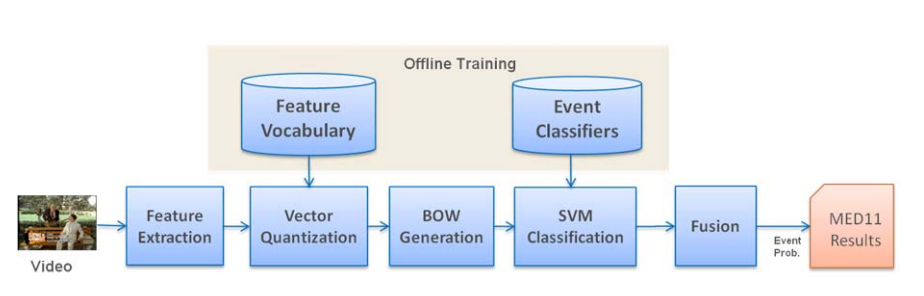
\includegraphics[width = \textwidth]{papergrafik.png}
	\caption{The processing pipeline of \cite{tamrakar2012evaluation}}
	\label{fig:grafik}
\end{figure}

\section{Results}

For each class, the first $2$ of the $45$ videos are taken for creating the clusters and the first $40$ videos are taken for training of the SVM.
The remaining $5$ videos, which are not used for training of the SVM are used for validation.

Overall precision of our classifier is $0.4$. Precision and recalls for each classes are as follows:
\begin{description}
    \item[Kiss] $p = 0.4, r = 0.4$
    \item[Handshake] $p = 0.5, r = 0.4$
    \item[High Five] $p = 0.66, r = 0.4$
    \item[Hug] $p = 0.25, r = 0.4$
\end{description}
Further details can be seen in Table \ref{tab:eval}.

\begin{center}
\begin{tabular}{l|l|c|c|c|c|c}    
    \multicolumn{2}{c }{}
        & \multicolumn{4}{c}{Prediction} & \\ \cline{3-6}
    \multicolumn{2}{c|}{}
        & Kiss & Handshake & High Five & Hug & \multicolumn{1}{c}{Total} \\ \cline{2-6}
    \multirow{4}{*}{Actual} 
        & Kiss      & $2$ & $1$ & $1$ & $1$ & $5$\\ \cline{2-6}
        & Handshake & $0$ & $2$ & $0$ & $3$ & $5$\\ \cline{2-6}
        & High Five & $1$ & $0$ & $2$ & $2$ & $5$\\ \cline{2-6}
        & Hug       & $2$ & $1$ & $0$ & $2$ & $5$\\ \cline{2-6}
    \multicolumn{1}{c}{} & \multicolumn{1}{c}{Total} 
        & \multicolumn{1}{c}{$5$} & \multicolumn{1}{c}{$4$} 
        & \multicolumn{1}{c}{$3$} & \multicolumn{1}{c}{$8$} & \multicolumn{1}{c}{$20$}\\
\end{tabular}
\captionof{table}{Table showing the confusion matrix for our classifier.}
\label{tab:eval}
\end{center}

\bibliographystyle{ieeetr}
\bibliography{main}\textbf{}

\end{document}